\documentclass[12pt]{article}
\usepackage{graphicx} % Required for inserting images
\usepackage{enumitem}
\usepackage{mathtools}
\usepackage{amsmath}
\usepackage{gvv-book}
\usepackage{gvv}

\title{\textbf{5.3.38}}
\author{\textbf{EE25BTECH11004 - Aditya Appana}}
\date{September 27, 2025}

\begin{document}

\maketitle

\section*{Question}
Find the value of $x$, if\\
$$3x+y=1$$
$$2y-x=-5$$

\section*{Solution}

Organizing the given equations into an augmented matrix:
\begin{align}
\myvec{3&1&1 \\ -1&2&-5}
\end{align}
Performing row operations:
\begin{align}
\myvec{3&1&1 \\ -1&2&-5}\xrightarrow{\text{R_1 \rightarrow $R_1- \frac{1}{2}R_2$}}   \myvec{\frac{7}{2}& 0 & \frac{7}{2} \\ -1 & 2 & -5} \\
\myvec{\frac{7}{2}& 0 & \frac{7}{2} \\ -1 & 2 & -5}  \xrightarrow{\text{R_2 \rightarrow $R_2+ \frac{2}{7}R_1$}} \myvec{\frac{7}{2}& 0 & \frac{7}{2} \\ 0 & 2 & -4} \\
\myvec{\frac{7}{2} & 0 & \frac{7}{2} \\ 0 & 2 & -4} \xrightarrow{\text{R_2 \rightarrow $R_2/2$}} \myvec{\frac{7}{2} & 0 & \frac{7}{2} \\ 0 & 1 & -2} 
\end{align}
\newpage
\begin{align}
\myvec{\frac{7}{2} & 0 & \frac{7}{2} \\ 0 & 1 & -2} \xrightarrow{\text{R_1 \rightarrow $2/7 R_1$}} \myvec{1& 0 & 1 \\ 0 & 1 & -2}
\end{align}

$x = 1$, $y=-2$

\begin{figure}[H]
    \centering
    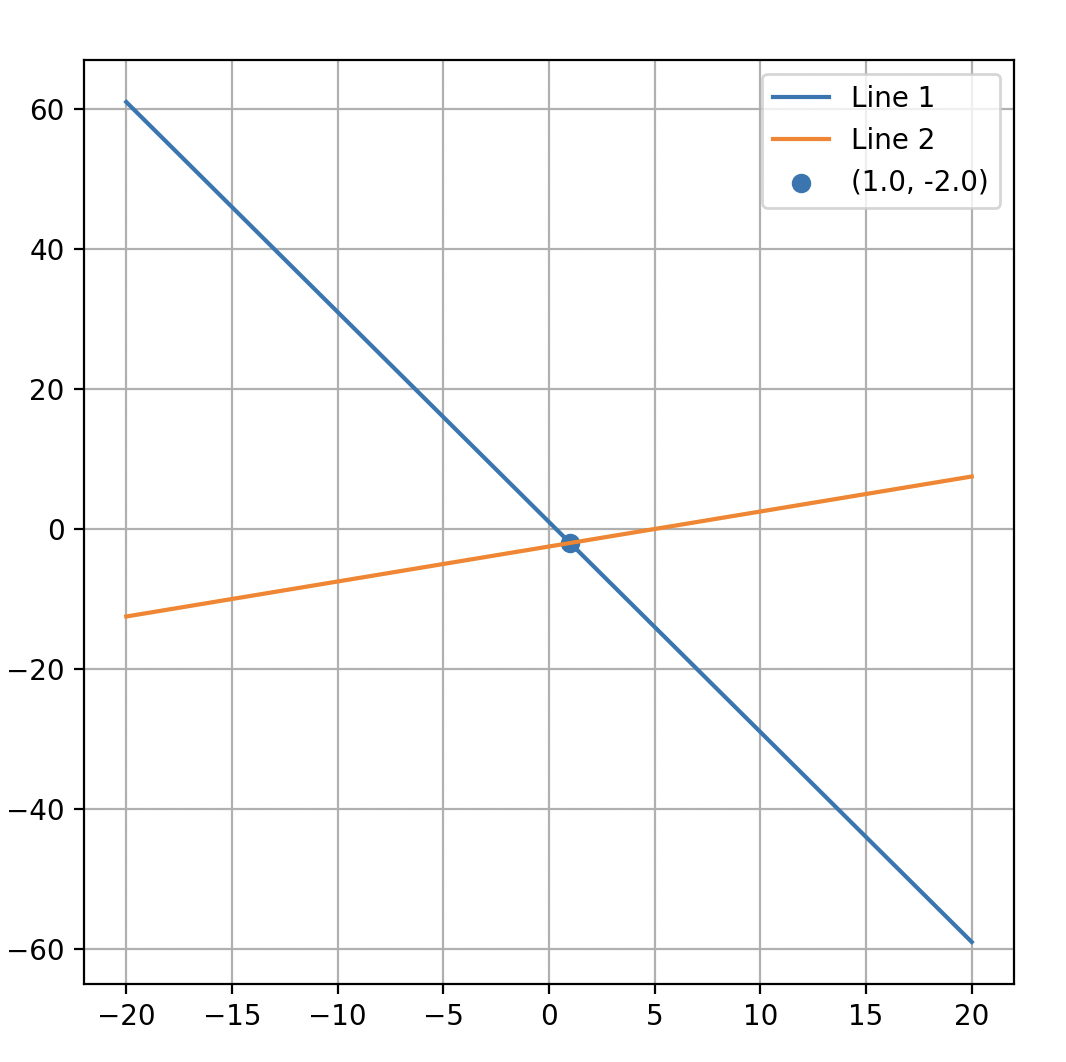
\includegraphics[width=0.6\columnwidth]{Figs/5338.png}
    \caption{Plot}
    \label{fig:placeholder}
\end{figure}
\end{document}